\section{Type inference}

We now formulate type inference for the \lang language. Type inference is
based on the HM(X) framework~\citep{DBLP:journals/tapos/OderskySW99} which
presents how to implement Hindley-Milner type inference in a language
with qualified types. We first present various preliminaries definitions,
we then show our extension of HM(X) that support a kind system and affine
types.

\subsection{Preliminaries}

\subsubsection{Constraint language}

\newcommand\A{\mathcal A}
\newcommand\SC{\mathcal S}

Let us note $\A$ our constraint system. The grammar of constraints is
given in  \cref{grammar:constraint}.
$\A$ is defined as the smallest cylindric term constraint system that
satisfies the axiom shown in \cref{rules:entail}.
We follows the traditional HM(X) formulation
with conjunctions, projections and type inequalities.
The new element specific to our approach are kind inequalities.
Entailment is noted $\entail{C}{D}$, where $D$ is a consequence of the
constraints $C$.
We say that $C$ and $D$ are equivalent, noted $C \equivC D$,
when $\entail{C}{D}$ and $\entail{D}{C}$.
\TODO{Give the cylindric properties ?}


\begin{figure}[tp]
  \centering
  \begin{align*}
    C &::= \Cleq{\tau_1}{\tau_2}
        \mid \Cleq{k_1}{k_2}
        \mid C_1 \Cand C_2
        \mid \Cproj{\tvar}{C}
        \mid \Cproj{\kvar}{C}
  \end{align*}
  \caption{The constraint language}
  \label{grammar:constraint}
\end{figure}

\begin{figure*}[tp]
  \begin{minipage}{0.65\linewidth}
  \begin{mathpar}
    \inferrule[Lat-UAL]{}{\kun \lk \kaff \lk \klin}
    \and
    \inferrule[Lat-Level]{\mul \lk \mul' \and n \lk n'}{\mul_n \lk_\Lat \mul'_{n'}}
  \end{mathpar}
\end{minipage}~
\begin{minipage}{0.2\linewidth}
  \centering
  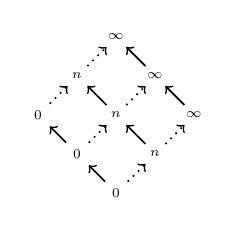
\begin{tikzpicture}
    [->,auto,semithick, every node/.style={scale=0.7}]
    \node(U) {$\kun_0$} ;
    \node(A) [above left of=U] {$\kaff_0$} ;
    \node(L) [above left of=A] {$\klin_0$} ;
    \node(Un) [above right of=U] {$\kun_n$} ;
    \node(An) [above left of=Un] {$\kaff_n$} ;
    \node(Ln) [above left of=An] {$\klin_n$} ;
    \node(Uinf) [above right of=Un] {$\kun_\infty$} ;
    \node(Ainf) [above left of=Uinf] {$\kaff_\infty$} ;
    \node(Linf) [above left of=Ainf] {$\klin_\infty$} ;
    \path
    (U) edge (A)
    (A) edge (L)
    (Un) edge (An)
    (An) edge (Ln)
    (Uinf) edge (Ainf)
    (Ainf) edge (Linf)
    ;
    \path[dotted]
    (U) edge (Un)
    (A) edge (An)
    (L) edge (Ln)
    (Un) edge (Uinf)
    (An) edge (Ainf)
    (Ln) edge (Linf)
    ;
  \end{tikzpicture}
\end{minipage}

%%% Local Variables:
%%% mode: latex
%%% TeX-master: "../main"
%%% End:

  \caption{Lattice inequalities -- $k \lk_\Lat k'$}
  \begin{mathpar}
  \inferrule
  {}{ \entail{}{\Cleq{\kvar}{\kaff}} }
  \and
  \inferrule
  {}{ \entail{}{\Cleq{\kun}{\kvar}} }
  \and
  \inferrule
  {}{ \entail{}{\Cleq{\kvar}{\kvar}} }
  \and
  % \inferrule
  % {\Cleq{k}{k'} \in C}{ \entail{C}{\Cleq{k}{k'}} }
  % \and
  % \inferrule
  % { \entail{C}{\Cleq{x_1}{x}}\\
  %   \entail{C}{\Cleq{x}{x_2}}
  % }
  % { \entail{C}{\Cleq{x_1}{x_2}} }
  % \and
  % \inferrule
  % { \entail{C}{D} }
  % { \entail{C}{\Cproj{x}{D}} }
  % \\
  \inferrule
  { \entail{C}{\Cleq{\tau'_1}{\tau_1}}\\
    \entail{C}{\Cleq{\tau_2}{\tau'_2}}\\
    \entail{C}{\Cleq{k}{k'}}
  }
  { \entail{C}{\Cleq{\tau_1\tarr{k}\tau_2}{\tau'_1\tarr{k'}\tau'_2}} }
  \and
  \inferrule
  { \forall i,\ \entail{C}{\Cleq{\tau_i}{\tau_i}}\\
  }
  { \entail{C}{\Cleq{\tapp{t}{(\tau_i)}}{\tapp{t}{(\tau'_i)}}} }
  \and
  
  % \and
  % \inferrule
  % { \entail{C}{\Cleq{k}{k'}} \\
  %   \entail{C}{\Cleq{k'}{k}} }
  % { \entail{C}{\Ceq{k}{k'}} }
  % \and
  % \inferrule
  % { \entail{C}{\Cleq{k}{k'}} }
  % { \entail{C}{\Ckind{\tau_0\tarr{k}\tau_1}}{k'}}
  % \and
  % \text{Completion to form a cylindric constraint system.}
\end{mathpar}

%%% Local Variables:
%%% mode: latex
%%% TeX-master: "../main"
%%% End:

  \caption{Base entailment rules -- $\entail{C}{D}$ }
  \label{rules:entail}
\end{figure*}


We note $\SC$ the set of solved forms
which can be used inside type and kind schemes.
We define $\SC$ as $\A$ quotiented by the relation $\equivC$.
%
We consider the existence of a function $\operatorname{normalize}$ which takes
a constraint in $\A$ and a substitution $\psi$ and returns a constraint
in solved form $C' \in \SC$,
and an updated substitution. We detail the implementation
of the normalization function in \cref{sec:normalize}

% $\mathcal S$ is composed only of kind
% inequalities \emph{over variables}. For convenience, if $C\in\mathcal S$, we
% note $C$ as a list of kind inequalities: $\Cleq{\kvar_i}{\kvar_{i'}}^n$.
% \TODO{Extend the properties of solved forms}



\subsubsection{Usage maps}

In order to determine if a variable is used in an affine manner, we must track
its uses and the associated kinds. For instance, in the expression
$(x,x)$, $x$ is used twice. If $x$ is of type $\tau$, which is of kind $k$,
we must add the constraint $\Cleq{k}{\kun}$. In order to record uses and kinds,
our type inference relation will return a ``usage map'', noted $\Sv$,
which associates each variable to a list of kinds corresponding to each use site
of the variable.
We note $\Sone{x}{k_1,\dots,k_n}$ the singleton usage map.
Common operations on usage maps are defined in \cref{op:usgmap}. We define
regular set operations such as union
($\Sv\cup\Sv'$) and intersection ($\Sv\cap\Sv'$), along
with constraint creation $\Cleq{\Sv}{k_0}$ which indicates that all the kinds
presents in the usage map $\Sv$ are constrained by the kind $k_0$.
These operations corresponds roughly to the various parts of the join
operator on sets $\esplit{}{}$.

\begin{figure}[tp]\centering
\begin{mathpar}
  % \Sv\cap\Sv'
  % &= \left\{ x \to l,l'
  %   \mid \Sone{x}{l}\in\Sv \text{ and } \Sone{x}{l'}\in\Sv' \right\} \\
  \infer
  { \forall x \in \Dom{\Sv_1}\cup\Dom{\Sv_2}.\quad
    \tsplit{C_x}{\Sv(x)}{\Sv_1(x)}{\Sv_2(x)}
  } 
  { \tsplit{(\bigwedge C_x)}{\Sv}{\Sv_1}{\Sv_2} }
  % &= \Sv\cap\Sv' \sqcup
  %   (\Sv\Sdel{x' \mid x'\in\Sv'}) \sqcup
  %   (\Sv'\Sdel{x \mid x\in\Sv})
  %   &\text{where $\sqcup$ is the disjoint union}\\
  \and
  \inferrule{}
  { \Cleq{\Sv}{k_0}
    = \bigwedge_{\Sone{x}{l_x}\in\Sv} \bigwedge_{k\in l_x} \Cleq{k}{k_0}
  }
  \and
  \inferrule
  { \forall \bshadow{x} \in \Sv, b'\in\Sv'.\quad
    \tregion{C_x}{y}{\bshadow{x}}{b'} }
  { \tregion{(\bigwedge C_x)}{y}{\Sv}{\Sv'} }
  \and
  % \inferrule
  % { \text{if } \operatorname{lenght}(\Sv(x))  = \Cempty{} \wedge  }
  { \Weaken_{(x,k)}(\Sv) =
    \begin{dcases}
      \Ctrue& \operatorname{length}(\Sv(x)) = 1\\
      {k}\lk\kaff_\infty& \text{ otherwise}\\
    \end{dcases}

  }
\end{mathpar}
\caption{Operation on usage maps $\Sv$}
\label{op:usgmap}
\end{figure}

\subsection{Kind inference}

We note $\inferK{(C,\unif)}{\bf{\E}}{\bf{\tau}}{k}$ when type $\tau$ has kind $k$
in environment $\E$ under constraints $C$ and unifier $\unif$. From an
algorithmic point of view, $\E$ and $\tau$ are the input parameters of
our inference procedure.
We present the kind inference algorithm as a set of syntax-directed rules in
\cref{rules:kinding}.
Since higher-kinded types are not supported, the type application
rule and the type constructor rule are merged in {\sc KApp}.
Additionally, type variables must be of a simple kind in rule {\sc KVar}.
Note that in the case of a type constructor with no argument, the {\sc KApp}
rule degenerates to a simpler form which is similar to the {\sc KVar} rule.
Kind schemes are instantiated in the {\sc KApp} and {\sc KVar} rules by creating
fresh kind variables and the associated substitution.

\begin{figure}[ht]
  \centering
  \begin{mathpar}
  \inferrule[KVar|KCons]
  { \bvar{\tvar|\T t}{
      \forall \kvar_i.\ \qual{D}{(\Multi[j]{k}) \karr k}}
    \in \E \\
    \Multi[i]{\kvar'} \text{ fresh} \\\\
    (C,\unif) =
    \normalize{D}{\subst{\kvar_i}{\kvar'_i}{}_i}
  }
  { \inferK{(C,\unif|_{\fv{\E}})}{\E}{\tvar|\T t}{\unif ((\Multi[j]{k}) \karr k)} }
  \and
  \inferrule[KArr]
  { }
  { \inferK{(\Ctrue,\emptyset)}{\E}{\tau_1 \tarr{k} \tau_2}{k} }
  \and
  \inferrule[KBorrow]
  { }{ \inferK{(\Ctrue,\emptyset)}{\E}{\borrowty{k}{\tau}}{k}}
  \and
  \inferrule[KApp]
  { \forall j,\
    \inferK{(C_j,\unif_j)}{\E}{\tau_j}{k'_j} \\
    \inferK{(C_0,\unif_0)}{\E}{\T t}{(\Multi[j]{k}) \karr k}
    \\\\
    (C,\unif) =
    \normalize
    {C_0\Cand \Multi[j]{C} \Cand \Multi[j]{\Ceq{k'_j}{k_j}}}
    {\unif_0\meet \Multi[j]{\unif}}
  }
  { \inferK{(C,\unif|_{\fv{\E}})}{\E}{\tapp{\tcon}{\Multi[j]{\tau}}}{\unif k} }
  \and
  \inferrule[KPair]
  { \forall i,\
    \inferK{(C_i,\unif_i)}{\E}{\tau_i}{k_i} \\
    \kvar \text{ fresh} \\\\
    (C,\unif) =
    \normalize
    {\Multi[i]{C} \Cand \Multi[i]{\Cleq{k_i}{\kvar}}}
    {\Multi[i]{\unif}}
  }
  { \inferK{(C,\unif)}{\E}{\tyPair{\tau_1}{\tau_2}}{\unif\kvar} }
\end{mathpar}


%%% Local Variables:
%%% mode: latex
%%% TeX-master: "../main"
%%% End:

  \caption{Kind inference algorithm -- $\inferK{(C,\unif)}{\E}{\tau}{k}$}
  \label{rules:kinding}
\end{figure}

\begin{figure}[ht]
  \centering
  \begin{mathpar}
  \inferrule[KVar]
  { \bvar{\tvar}{k} \in \E }
  { \inferSK{C}{\E}{\tvar}{k}
  }
  \and
  \inferrule[KPair]
  { \forall i \quad
    \inferSK{C}{\E}{\tau_i}{k_i} \quad
    \inferSS{C}{\E}{k_i}{k}
  }
  { \inferSK{C}{\E}{\tyPair{\tau_1}{\tau_2}}{k} }
  \and
  \inferrule[KApp]
  { \bvar{\T{\tcon}}{
      \forall \Multi[i]\kvar.\ \qual{D}{(\Multi[j]{k'}) \karr k'}}
    \in \E \\
    \unif = \subst{\Multi[i]\kvar}{\Multi[i]k}{} \\
    \entail C {\unif D} \\
    \forall j\quad
    \inferSK{C}{\E}{\tau_j}{k_j}\quad
    \inferSS{C}{\E}{k_j}{\unif{k'_j}}
  }
  { \inferSK{C}{\E}{\tapp{\tcon}{\Multi[j]{\tau}}}{\unif{k'}} }
  \and
  \inferrule[KBorrow]
  {}{ \inferSK{C}{\E}{\borrowty{k}{\tau}}{k}}
  \and
  \inferrule[KArr]
  {}
  { \inferSK{C}{\E}{\tau_1 \tarr{k} \tau_2}{k} }
\end{mathpar}


%%% Local Variables:
%%% mode: latex
%%% TeX-master: "../main"
%%% End:

  \caption{Syntax-directed kind inference -- $\inferSK{C}{\E}{\tau}{k}$}
  \label{rules:sd-kinding}
\end{figure}


\subsection{Type inference}

We reformulate the HM(X) type inference in the context of our affine type
system. The main difference compared to HM(X) are noted in \addlin{blue}.
We note $\inferW{\addlin{\Sigma}}{(C,\unif)}{\bf{\E}}{\bf{e}}{\tau}$ when
$e$\ as type $\tau$ in $\E$ under the constraints $C$ and unifier $\unif$.
$\Sigma$ is a map which associates free variables in $e$ to
their kinds.
As before, $\E$ and $e$ are the input parameters of the inference
algorithm. The syntax-directed rules are shown in \cref{rules:typing}.

\begin{figure*}[h]
  \begin{mathpar}
  \ruleIVar
  
  \ruleIBorrow
  \\
  \ruleIAbs
  
  \ruleIReBorrow
  \\
  \ruleIApp
  
  \ruleIRegion

  \ruleIMatch

  \ruleIPair

  \ruleILet

  { \Weaken_{\bvar{x}{\sigma}}(\Sv) =
    \begin{dcases}
      \Ctrue& \text{if } x\in\Sv\\
      \Cleq{\sigma}{\kaff_\infty}&\\
    \end{dcases}
  }
\end{mathpar}

% \begin{align*}
%   \Weaken(x,\Sv)
%   &\equiv \begin{cases}
%     \operatorname{kind}(x)\lk\kun &\text{if } \operatorname{kind}(x)\in\Sv\\
%     \Cempty &\text{otherwise}
%   \end{cases}\\
%   \Cleq{\Sv}{k}
%   &\equiv \bigwedge_{\kvar\in\Sv} \Cleq{\kvar}{k}
% \end{align*}

%%% Local Variables:
%%% mode: latex
%%% TeX-master: "../main"
%%% End:

  \caption{Type inference algorithm -- $\inferW{\Sigma}{(C,\psi)}{\bf{\E}}{\bf{e}}{\tau}$ }
  \label{rules:typing}
\end{figure*}

\begin{figure*}[ht]
  \begin{mathpar}
  \inferrule[Scheme]{
    \inferSK{C \Cand C_x} \E \tau {k'} \\
    \entail C {\Cleq{k'}k}
  }{
    \entail C {(\forall \kvar_i \forall (\tvar_j:k_j).\
      \qual{C_x}{\tau}) \le  k}
  }
\end{mathpar}
\hrulefill
\begin{mathpar}
  \inferrule[Var]
  { \bvar{x}{
      \forall \kvar_i \forall (\tvar_j:k_j).\ \qual{C_x}{\tau}
    }
    \in \E \\
    \unif = [\kvar_i\mapsto k_i,\tvar_j \mapsto \tau_j] \\
    \entail C {\unif(C_x)} \\
    % \addlin{
    %   \inferSK{C}{\E}{\unif \tau}{k_\tau}
    % }
  }
  { \inferS{C}{\E}{x}{\unif\tau}
  }
  \and
  \ruleSDLam
  \and
  \ruleSDApp
  \and
  \inferrule[Let]
  { \inferS{C \Cand D}{\E_1}{e_1}{\tau_1} \\
    \schm = \forall\Multi\kvar\forall\bvar{\Multi\tvar}{\Multi{
        k}}. \qual{D}{\tau_1}\\
    \{\Multi\kvar, \Multi\tvar\} = \fv{D, \tau_1} \setminus \fv{C, \E}
  \\
  \entail{C}{\exists\Multi\kvar\Multi\tvar.D} \\
    \inferS{C}{\E;\bvar{x}{\sigma}}{e_2}{\tau_2} \\
    \addlin{\lsplit{C}{\E}{\E_1}{\E_2}}\\
  }
  { \inferS{C}
    {\E}{\letin{x}{e_1}{e_2}}{\tau_2} }
  \and
  \inferrule[Pair]
  { \inferS{C}{\E_1}{e_1}{\tau_1} \\
    \inferS{C}{\E_2}{e_2}{\tau_2} \\
    \addlin{\lsplit{C}{\E}{\E_1}{\E_2}}
  }
  { \inferS{C}{\E}{\introPair{e_1}{e_2}}{\tyPair{\tau_1}{\tau_2}} }
  \and
  \inferrule[MatchPair]
  { 
    \inferS{C}{\E_1}{e_1}{\tyPair{\tau_1}{\tau'_1}} \\
    \inferS{C}
    {\E_2;\bvar{x}{\tau_1};\bvar{x'}{\tau'_1}}{e_2}{\tau_2} \\
    \addlin{\lsplit{C}{\E}{\E_1}{\E_2}}
  }
  { \inferS{C}
    {\E}{\matchin{x,x'}{e_1}{e_2}}{\tau_2} }
  \and
  %
  \inferrule[Borrow]
  { 
    \bvar{\borrow x}{\borrowty k\tau} \in \E
  }
  { \inferS{C}{\E}{\borrow{x}}{\borrowty{k}{\tau}} }
  \and
  \inferrule[Region]
  { \svar x {\tau_x} \in \E \\
    \addlin{ \bregion{C_r}{x}{\E}{\E'} }\\
    \inferS{C}{\E'}{e}{\tau} \\
    \inferSK{C}{\E}{\tau}{k_\tau}\\
    \entail C {\Cleq{k_\tau}{\klin_{n-1}}} \\
  }  { \inferS{C}{\E}{\region{x}{e}}{\tau} }
  \and
  %
  % \inferrule[Elim]
  % { \tvar,(\kvar'_i),(\tvar'_j)\text{ new}\\
  %   \bvar{K}{
  %     \forall \kvar_i \forall (\tvar_j:\kvar_j).\ \qual{C_K}{\tau_1 \tarr{}\tau_2}
  %   } \in \E\\
  %   \inferW{\Sv}{(C,\unif)}{\E}{e}{\tau} \\
  %   \unif' =
  %   \subst{\kvar_i}{\kvar'_i}{} \meet
  %   \subst{\tvar_j}{\tvar'_j}{} \meet \unif \\
  %   D =
  %   C \Cand C_K \Cand \Cleq{\tau_1}{\tvar} \Cand \Cleq{\tau}{\tau_2} \\
  %   (C,\unif) = \normalize{D}{\unif'}\\
  % }
  % { \inferW{\addlin{\Sv}}{(C,\unif|_{\fv{\E}})}{\E}{\elimK{K}{e}}
  %   {\unif\tvar} }
\end{mathpar}

% \begin{align*}
%   \Weaken(x,\Sv)
%   &\equiv \begin{cases}
%     \operatorname{kind}(x)\lk\kun &\text{if } \operatorname{kind}(x)\in\Sv\\
%     \Cempty &\text{otherwise}
%   \end{cases}\\
%   \Cleq{\Sv}{k}
%   &\equiv \bigwedge_{\kvar\in\Sv} \Cleq{\kvar}{k}
% \end{align*}

%%% Local Variables:
%%% mode: latex
%%% TeX-master: "../main"
%%% End:

  \caption{Syntax-directed typing rules}
  \label{fig:syntax-directed-typing}
\end{figure*}
\subsection{Normal forms and generalization}
\label{sec:normalize}


We now place ourselves in a more general context where kinds are either variables
or constants belonging to a total bounded lattice $(\mathcal L, \lk_\Lat)$ ie.,
a lattice which admits a total order and upper and lower bounds ($l^\top$ and $l^\bot$).
We note lattice elements $l$ and $\glb_i l_i$ (resp. $\lub_i l_i$)
the greatest lower bound (resp. least upper bound) in $\mathcal L$.
%
Let $\CL$ the set of constraints in this lattice. We consider the
following base entailment rules in this system:
\begin{center}
  \begin{mathpar}
    \inferrule{l \lk_\Lat l'}{\entail{}{\Cleq{l}{l'}}}
    \and
    \inferrule{}{\entail{}{\Cleq{k}{l^\top}}}
    \and
    \inferrule{}{\entail{}{\Cleq{l^\bot}{k}}}
  \end{mathpar}
\end{center}



The normalization procedure is noted $\normalize{C_0}{\unif_0}$ where
$C_0\in \CL$ is a set of constraints and $\unif_0$ is a substitution.
It returns a constraint $C \in \mathcal S$ in
solved form and a unifier $\unif$.
The main idea of the algorithm is to first remove all the type equalities
by using regular Herbrand unification. After that, we only have
a set of inequalities among kinds, which we can consider as a relation.
We can then saturate the relation,
unify all kinds that in the same equivalence classes to obtain
a most general unifier on kind variables,
remove all existentially quantified variables and
then minimize back the relation.

More precisely, we apply the following steps:
\begin{enumerate}
\item Solve all type equality constraints through Herband unification and
  gather all existential quantifications at the front of the constraint.
  We obtain a constraint $C^k = \exists \kvar_i,\ \Cleq{k_j}{k'_j}_j$ and
  a substitution $\unif_\tau$.
  
  We note $\mathcal R$ the relation $\Cleq{k_j}{k'_j}_j$,
  $\mathcal G$ the underlying directed graph and $V$ its vertices.

\item Saturate the lattice equalities in $\mathcal R$.
  
  More precisely, for each kind variable $\kvar \in V$,
  for each constant $l_i$ (resp. $l_j$) such that
  there is a path from $l_i$ to $\kvar$ (resp. from $\kvar$ to $l_j$) in $\mathcal G$,
  add an edge from $\lub l_i$ to $\kvar$
  (resp. from $\kvar$ to $\glb l_j$).
  This step is well defined since $\mathcal L$ is a bounded lattice
  and $\lub\emptyset$ and $\glb\emptyset$ are well defined.

  We also complement $\mathcal R$ with $(\leq)$ by adding an edge
  between related constants.
\item
  At this point, we can easily check for satisfiability: A constraint
  is satisfiable (in the given environment) if and only if,
  for any constants $l_1$ and $l_2$ such that
  there is a path from $l_1$ to $l_2$ in $\mathcal G$, then $l_1\lk_\Lat l_2$.
  If this is not the case, we return \textbf{fail}.
  
\item For each strongly connected component in $\mathcal G$, unify all its vertices and replace it by a representative.
  We note $\unif_k$ the substitution that replaces a kind variable by
  its representative.
  The representative of a strongly connected component $g$ can be determined as follows:
  \begin{itemize}
  \item If $g$ does not contain any constant, then the representative
    is a fresh kind variable.
  \item If $g$ contains exactly one constant, it is the representative.
  \item Otherwise, the initial constraint $C_0$ is not satisfiable.
  \end{itemize}
  Note that this step will also detect all unsatisfiable constraints.
\item Take the transitive closure of $\mathcal R$.
\item Remove all the vertices corresponding to the kind variables $\kvar_i$
  that are existentially quantified in $C^k$.
\item Take the transitive reduction of $\mathcal R$.
\item Remove the extremums of $\mathcal L$ and the edges of $(\leq)$
  from $\mathcal R$.
\item Return $C = \left\{ k \leq k' \mid k \operatorname{\mathcal R}k' \right\}$
  and $\unif =  \unif_\tau \meet \unif_k$.
\end{enumerate}

\TODO{Add an example}

\subsubsection{Soundness and Principality}

\begin{lemma}[Normal form]
  \label{lemma:normalform}
  Given a constraint $D\in\CL$, a substitution $\phi$ and
  $(C,\unif) = \normalize{D}{\phi}$,
  then $\phi\leq\unif$,
  $C \equivC \unif D$ and
  $\unif C = C$.
\end{lemma}
\begin{proof}
  % For simplicity, we assume that any substitution has been already applied
  % to $D$ and that $\phi = id$.
  Let us partition $\phi$ into a part which affects type variables,
  $\phi_\tau$, and a part which affects kind variables, $\phi_k$.
  
  We note $(C^k,\unif_\tau)$ the result of
  the modified Herbrand unification on $(D,\phi)$ in step (1).
  Herbrand unification computes the most general
  unifier. Our modified Herbrand unification only output additional
  kind constraints for kind on the arrows and does not change
  the result of the unification. Thus, we have
  $\phi_\tau\leq\unif_\tau$,
  $C^k \equivC \unif_\tau D$ and
  $\unif_\tau C^k = C^k$.
  
  Let $C^{k+}$ be the result after step (2), we trivially have that
  $\fv{C^{k+}} = \fv{C^k}$ and that $C^{k+} \equivC C^k$.

  Let $C^{A}$ and $\unif_k$ be the results after step (4).
  By definition, we have $\unif_k C^{k+} \equivC C^{A}$ and
  $\unif_k C^{A} = C^{A}$. Since $\phi_k$ has already be applied to $C$ before
  unifying the strongly connected components,
  we have that $\phi_k\leq\unif_k$.

  Let $\unif = \unif_\tau \meet \unif_k$. Since $\unif_\tau$ and $\unif_k$
  have disjoint supports,
  we have $C^{A} = \unif_\tau C^{A} \equivC \unif C^{k+} \equivC \unif D$
  and $\unif C^{A} = C^{A}$.
  Furthermore, $\phi_\tau \meet \phi_k \leq \unif_\tau \meet \unif_k$.
  
  Steps (5) to (9) all preserve the free variables and the equivalence
  of constraints, which concludes.
\end{proof}

\begin{lemma}[Uniqueness]
  Given $(C_1,\unif_1)$ and $(C_2,\unif_2)$ such that
  $\unif_1 C_1 \equivC \unif_2 C_2$, then
  $\normalize{C_1}{\unif_1}$ and $\normalize{C_2}{\unif_2}$
  are identical up to $\alpha$-renaming.
\end{lemma}
\begin{proof}
  In \cref{lemma:normalform}, we have showed that all the steps of the
  normalization procedure preserve equivalence.
  Since $\unif_1 C_1 \equivC \unif_2 C_2$, equivalence between
  the two results of the normalization procedures is preserved for all steps.

  We note $P(C_a)$ if for all $C = (k, k)'$
  such that $\entail{C_a}{C}$ and $\nvdash_eC$,
  we have $C \in {\mathcal R}_a$. 

  Let us note $C_1'$ and $C_2'$ the constraints after step (4). $P(C_1')$ and
  $P(C_2')$ hold. Indeed, since $C_1'$ and $C_2'$ are only composed
  of existential quantifications and kind inequalities, the only rules
  that applies are transitivity and lattice inequalities.
  After step (2) and (5), the associated relations are fully saturated for these
  two rules, hence all inequalities that can be deduced from $C_a'$ are already
  present in the relation.

  The property $P$ is preserved by step (6) since we only remove
  inequalities that involve existentially quantified variables. Such
  inequalities could not be picked in $P$.
  % In (6) we only remove
  % trivial lattice inequalities.

  Let us note $C''_a$ for $a\in\{1,2\}$ the constraints after step (5).
  Since there are no more existential variables,
  we have $C''_a=(k_i,k'_i)_i=\mathcal R''_a$.
  For any $C=(k,k')$ such that $\entail{}{C}$ and $\entail{C''_a}{C}$,
  then $C \in (\leq) \subset {\mathcal R}''_a$.
  Indeed, the only trivial inequalities in our system are equalities of the form
  $(\kvar, \kvar)$, which were removed in step (4) and the lattice inequalities.

  Let us consider $C = (k,k') \in \mathcal R''_1$.
  Since $C''_1\equivC C''_2$, we have $\entail{C''_2}{C}$.
  If $\nvdash_e{C}$, by $P(C''_2)$ we have that
  $C\in R''_2$.
  If $\entail{}{C}$, then $C\in (\leq) \subset R''_2$.
  We conclude that $R''_1 \subset R''_2$.
  By symmetry, $R''_1 = R''_2$ and $C''_1 = C''_2$.

  This equality is preserved by step (7) and (8)
  since the transitive reduction of a directed acyclic graph is unique,
  which concludes.
\end{proof}


\begin{theorem}
  $\CL$ has the principal constraint property and
  $\operatorname{normalize}$ computes principal normal forms for $\CL$.
\end{theorem}

\begin{lemma}
  For all $C\in\mathcal S$, $\entail{C}{x = x}$ implies
  $\entail{}{x = x}$.
\end{lemma}
\begin{proof}
  By definition of $\operatorname{normalize}$, We have $C = \Cleq{k}{k'}_i$
  such that the underlying relation has no cycles.
  Thus, we can not deduce neither kind nor type equalities from $C$.
\end{proof}

\begin{lemma}
  $\CL$ is regular, ie, for $x, x'$ two types or kinds,
  $\entail{}{\Ceq{x}{x'}}$ implies
  $\fv{x} = \fv{x'}$
\end{lemma}
\begin{proof}
  The only equalities possibles are between variables (via symmetry) or
  between constants.
\end{proof}

\begin{theorem}
  Type inference in $HM(\CL)$ is sound, principal and complete.
\end{theorem}


\subsection{Principality}

\TODO{}

\begin{itemize}
\item Properly ensure that it respects HM(X) (cylindric, \dots)
\item Show principal type inference:
  \begin{itemize}
  \item Principal constraint system
  \item Regular constraint system: $\Ceq{\tau}{\tau'} \implies \fv{\tau} = \fv{\tau'}$.
  \item Solved forms are in simplified form.
    $C\in S, \entail{C}{\Ceq{\tau}{\tau'}} \implies \entail{}{\Ceq{\tau}{\tau'}}$.
  \end{itemize}
\item Show equivalence with the logic-based system.

\end{itemize}


% \begin{lemma}
%   Without loss of generality, we can consider that
%   kind inequalities in satisfiable constraints
%   are only done on kind variables. 

%   \begin{proof}
%     Consider the constraint $\Cleq{k}{k'}\Cand C$.
%     \begin{itemize}
%     \item If $k$ and $k'$ are both constants, it can be removed.
%     \item If the constraint is $\Cleq{\kvar}{\kaff}$ or $\Cleq{\kun}{\kvar}$, it can be removed.
%     \item If the constraint is $\Cleq{\kvar}{\kun}$ or $\Cleq{\kaff}{\kvar}$, we
%       can substitute $\kvar$ by its value in $C$.
%     \end{itemize}
%   \end{proof}
% \end{lemma}

%%% Local Variables:
%%% mode: latex
%%% TeX-master: "../main"
%%% End:
